\documentclass{article}

% NeurIPS 2026 Position Paper Track
\usepackage[position]{neurips_2026}

% Standard NeurIPS packages
\usepackage[utf8]{inputenc}
\usepackage[T1]{fontenc}
\usepackage{hyperref}
\usepackage{url}
\usepackage{booktabs}
\usepackage{amsfonts}
\usepackage{nicefrac}
\usepackage{microtype}
\usepackage{xcolor}
\usepackage{graphicx}
\usepackage{multirow}

% Colored prompt boxes
\usepackage[most]{tcolorbox}

\definecolor{PromptBlue}{HTML}{F3F8FF}
\definecolor{PromptFrame}{HTML}{2F5D9B}
\definecolor{PromptTitle}{HTML}{E7F0FF}

\newtcolorbox[auto counter]{promptbox}[2][]{
  enhanced,
  colback=PromptBlue,
  colframe=PromptFrame,
  coltitle=black,
  colbacktitle=PromptTitle,
  title={Prompt~\thetcbcounter: #2},
  fonttitle=\bfseries\small,
  fontupper=\small,
  boxrule=0.5pt,
  arc=1.2mm,
  left=1.2mm,
  right=1.2mm,
  top=1mm,
  bottom=1mm,
  toptitle=0.7mm,
  bottomtitle=0.7mm,
  attach boxed title to top left={xshift=1.5mm,yshift=-1.2mm},
  boxed title style={
    boxrule=0pt,
    arc=1mm,
    left=1mm,
    right=1mm,
    top=0.4mm,
    bottom=0.4mm
  },
  #1
}

\title{Population Modeling Should Be First-Order in LLM-Based Survey Simulation}

% Anonymous submission — do not include author names or affiliations
\author{
  Anonymous Author(s)
}

\begin{document}

\maketitle

\begin{abstract}
LLM-based survey simulation is often treated as a problem of generating more realistic
synthetic respondents. \textbf{We argue instead that population modeling should be a
first-order design problem in LLM-based survey simulation.} A survey measures a target
population, an LLM reflects an implicit model population, and external domain evidence
provides an observed but biased mediator population. Using a real world large scale Chinese consumer-health
survey benchmark and a domain-matched corpus of
nearly half a million online posts from Sina Weibo and Xiaohongshu, we compare semantic mapping and LLM simulation under
post-level and population-structured aggregation. Across both estimator families,
recovering candidate mediator units before aggregation improves alignment with real
survey distributions. These results suggest that survey-simulation research should
report not only the model, prompt, or estimator, but also which population is being
represented, what mediator evidence is used, and what population unit supports inference.
\end{abstract}

\section{Introduction}

LLM-based survey simulation has recently emerged as a promising tool for approximating
public opinion, consumer preferences, and population-level behavior. Researchers have
prompted large language models (LLMs) to answer surveys as synthetic respondents,
personas, or demographic groups, and have shown that these simulations can sometimes
reproduce aggregate patterns in human survey data~\cite{aher2023using,argyle2023silicon,santurkar2023whose,yang2024specializing}.
At the same time, domain-specific external evidence offers a way to ground these
simulations in observed patterns of language, behavior, experience, and preference.

However, current survey-simulation pipelines face a population-representation problem.
When an LLM is asked to answer a survey, its responses are shaped by the model's
training corpus, alignment behavior, and implicit assumptions about the target population.
When external evidence such as social media, online trace, or other domain-specific
observational data is used, it is often treated as an unstructured pool of observations,
even though such evidence is typically biased, heterogeneous, and organized around
distinct communities, contexts, and use cases.

\textbf{In this position paper, we argue that population modeling should be treated as a
first-order problem in LLM-based survey simulation: its reliability depends not only on
how survey answers are generated or estimated, but also on which population those
answers are intended to represent and what population unit the estimator operates on.}

We support this argument using a real-world Chinese consumer health survey and a
domain-matched corpus of Sina Weibo\footnote{\url{https://en.wikipedia.org/wiki/Weibo}} and Xiaohongshu\footnote{\url{https://en.wikipedia.org/wiki/Xiaohongshu}} posts. We organize the design space
along two dimensions: the response estimator, comparing semantic mapping with direct
LLM simulation; and the population unit, comparing post-level inference with
population-structured inference over recovered social-media groups. Across both response
estimators, we find that aggregating through latent social-media groups improves alignment
with real survey distributions. Finally, we conclude with a call for survey-simulation
research to treat population modeling as a first-order design problem, rather than relying
only on more realistic prompts or stronger language models.

\begin{figure}[htb!]
\centering
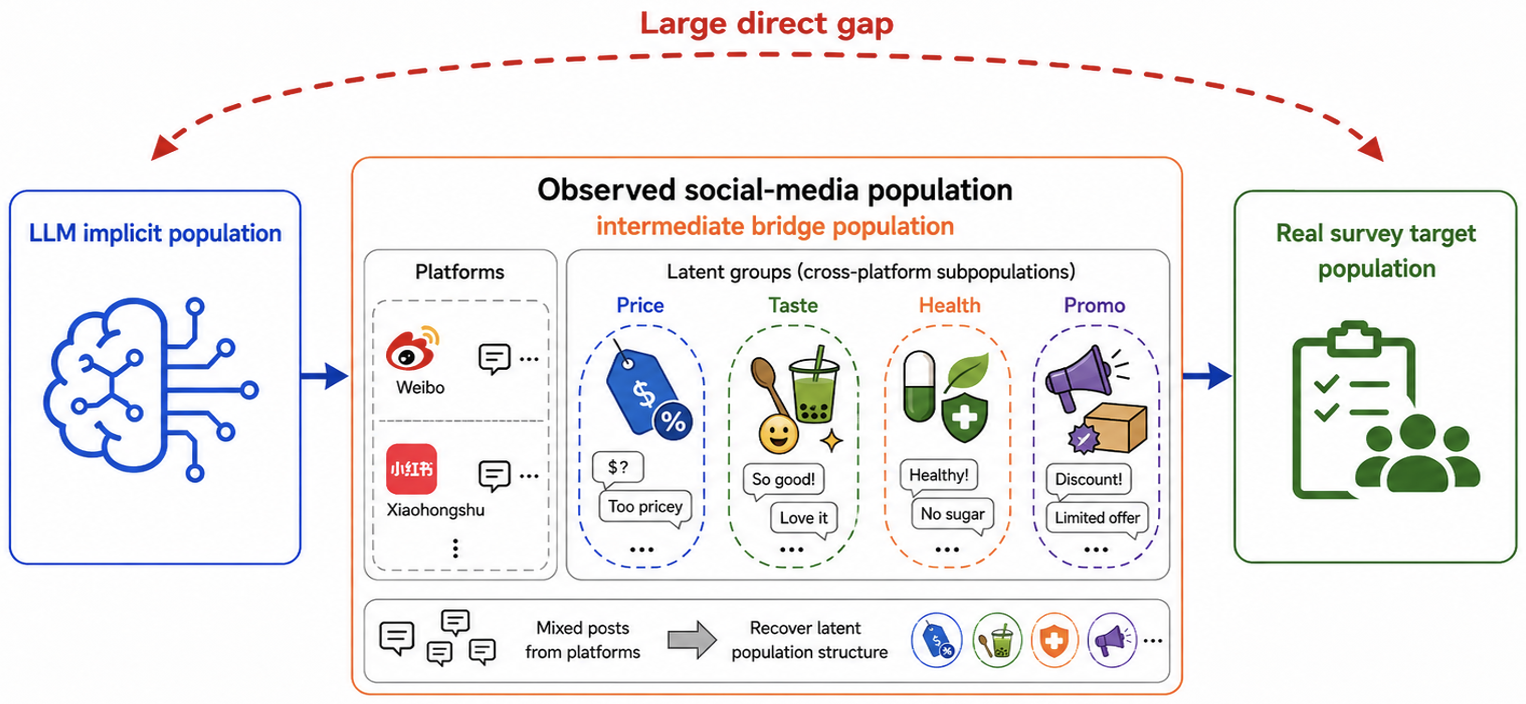
\includegraphics[width=0.9\linewidth]{bridge.png}
\caption{Population modeling with an observed mediator population. Survey simulation
requires relating the LLM's implicit population to the real survey target population
through an observed but biased mediator population. In our setting, this mediator is a
domain-specific social-media corpus.}
\label{bridge}
\end{figure}

\section{Related Work}

LLM-based survey simulation sits at the intersection of computational social science,
population modeling, and language technology. We organize prior work around three design
dimensions that are central to our argument: the \emph{response estimator}, or how
methods convert evidence into survey answers; the \emph{mediator population}, or what
observed evidence, if any, bridges the LLM and the target population; and the
\emph{population unit}, or what unit is simulated, inferred, and aggregated to form the
final distribution estimate. Different choices along these dimensions encode different
assumptions about which population is being represented. Making these choices explicit is
therefore necessary for diagnosing when and why survey simulation succeeds or fails.

\textbf{Response estimators.}
The dominant approach treats the LLM itself as the response estimator. ``Silicon samples''
and simulated-human-subject paradigms condition models on demographic profiles, personas,
or respondent descriptions, elicit answers, and aggregate them into survey distributions
\cite{argyle2023silicon,aher2023using}. Subsequent work shows both the promise and limits
of this strategy: LLMs can sometimes reproduce aggregate human patterns, but they also
reflect implicit demographic and cultural priors, flatten individual heterogeneity, and
fail under some inferential evaluations
\cite{santurkar2023whose,yang2024specializing,brand2023llms,park2024generative}.
Critical studies further show that plausible aggregate outputs can mask failures in
regression coefficients, response biases, and downstream social-science inference
\cite{bisbee2024synthetic,tjuatja2024do,ziems2024css}. A complementary line of work
replaces direct generation with semantic representation. Semantic Similarity Rating (SSR)
maps free-text responses to answer options through embedding similarity to reference
anchors, producing response distributions rather than single generated answers
\cite{maier2026llms}. Related critiques show that even non-generative mappings can carry
systematic calibration biases \cite{verap2026ssrbias}. Together, this literature suggests
that the response estimator is not a neutral implementation detail: it determines which
model assumptions enter the estimated survey distribution.

\textbf{Mediator populations.}
Early LLM survey simulation often places no external mediator between the model and the
target population; the model's training data, alignment, and default priors directly shape
the response distribution. Durmus et al.~\cite{durmus2023global}, for example, characterize
the LLM's implicit population by comparing model outputs with surveys from 65 countries
and find that default responses are closest to U.S.\ and Western European opinion. This
motivates methods that introduce external evidence to bridge the model and the target
population. One established approach uses demographic or census information as a structured
mediator: multilevel regression with post-stratification corrects non-representative
samples using population cell counts \cite{gelman1997poststratification,wang2015forecasting},
and recent LLM work extends this logic by constructing population-aligned personas or
using rich individual interviews as grounding evidence
\cite{hwang2023aligning,park2024generative}. Other work uses domain-specific online
evidence as an observed but biased mediator population. Such evidence can contain
survey-relevant signals, but it is also shaped by selection effects, platform dynamics,
and missing subgroups \cite{diaz2016online,sen2017total}. Recent systems prompt LLMs to
extract opinions from online text or use agentic pipelines to gather and aggregate such
signals \cite{cerina2024ai,surveypilot2024}. However, these approaches often treat the
mediator either as a flat pool of text or as a source requiring external demographic
correction, leaving its internal structure under-modeled.

\textbf{Population units.}
Every survey-simulation pipeline also makes an implicit choice about the unit of
inference. Persona-based methods typically operate at the individual level: one profile,
one simulated respondent, one response \cite{argyle2023silicon,aher2023using,brand2023llms}.
When richer individual evidence is available, such as interview transcripts, individual
agents can become substantially more accurate \cite{park2024generative}; when demographic
structure is known, methods can instead aggregate through strata or persona mixtures
weighted to match a target population
\cite{gelman1997poststratification,wang2015forecasting,hwang2023aligning,wang2024mixture}.
A shared assumption across much of this work is that the relevant population structure is
known in advance or can be defined by demographic categories. In many domains, however,
the available mediator evidence is organized around communities, topics, use contexts, or
behavioral situations rather than clean demographic cells. Our work therefore treats the
population unit as an empirical design choice: we recover candidate mediator units from
observed domain discourse and test whether aggregating through these units changes
alignment with real survey distributions. This supports a diagnostic question that prior
work rarely isolates: holding the response estimator fixed, does the population unit
change the estimated distribution?

\section{Problem Formulation and Design Space}
\label{sec:problem}

We study survey distribution estimation with three populations in mind:
the \emph{real survey population}, whose answer distribution is the target;
the \emph{LLM implicit population}, induced by the model's training data and alignment;
and an \emph{mediator population}, which is biased but domain-relevant.
Our goal is to use the observed mediator population as a mediator for estimating the real survey answer distribution.

For a survey question $q$ with answer options $\mathcal{Y}=\{1,\ldots,K\}$,
let $p^{\star}(y \mid q)$ denote the real survey distribution.
Given a social-media corpus $\mathcal{S}=\{s_i\}_{i=1}^{N}$,
we seek an estimator
\[
\hat{p}(y \mid q,\mathcal{S}) \approx p^{\star}(y \mid q).
\]

Given a mediator population, we organize the method space along two dimensions, shown in Figure~\ref{2by2}.
The first dimension is the \emph{response estimator}: how textual evidence is converted into a distribution over survey answers.
The second dimension is the \emph{population unit}: the unit over which response estimates are produced and aggregated.

\begin{figure}[htb!]
\centering
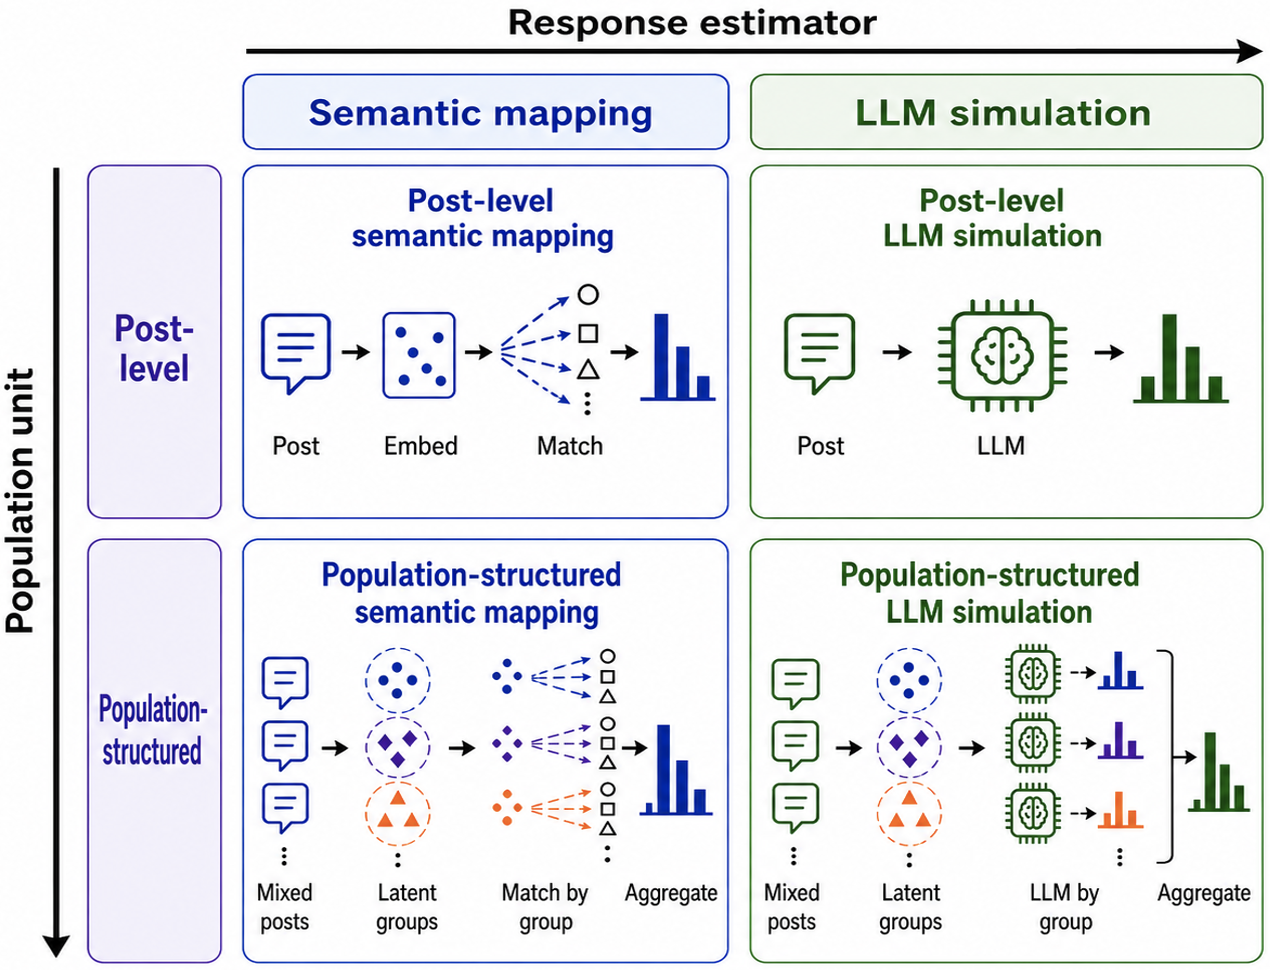
\includegraphics[width=0.65\linewidth]{2by2.png}
\caption{Two-by-two design space for LLM-based survey simulation.}
\label{2by2}
\end{figure}

\subsection{Response estimator}
A response estimator maps textual evidence $x$ to an answer distribution $f(y \mid q,x)$.
We consider two estimator families.
Semantic mapping estimates $f$ by comparing the semantic representation of $x$ with answer-option anchors.
LLM simulation estimates $f$ by prompting a language model to directly return a probability distribution over the answer options.
The detailed implementations are described in Sections~\ref{SSR_sec} and~\ref{LLM_prompt}.

\subsection{Population unit}
Under \emph{post-level inference}, each social-media post is treated as an independent unit:
\[
\hat{p}_{\mathrm{post}}(y \mid q,\mathcal{S})
=
\frac{1}{N}\sum_{i=1}^{N} f(y \mid q, s_i).
\]
This treats the observed corpus as a flat collection of posts.

Under \emph{population-structured inference}, the corpus is first organized into latent groups
$\mathcal{G}=\{G_1,\ldots,G_C\}$ with weights $\pi_c$ such that $\sum_{c=1}^{C}\pi_c=1$.
The final estimate aggregates group-level response distributions:
\[
\hat{p}_{\mathrm{struct}}(y \mid q,\mathcal{S})
=
\sum_{c=1}^{C} \pi_c \hat{p}_c(y \mid q,G_c).
\]
This treats social media as a structured mediator population rather than a flat sample.

Together, these dimensions define four practices:
post-level semantic mapping, population-structured semantic mapping,
post-level LLM simulation, and population-structured LLM simulation.
This design lets us separate errors due to response estimation from errors due to population representation.

\section{Experiment}
\label{sec:experiment}

We use the experiment to support the central position of this paper:
LLM-based survey simulation should be evaluated as a population-bridging problem,
not merely as a response-generation problem.
Accordingly, our empirical study is organized around three questions.
First, what real survey population are we trying to approximate?
Second, what observed social-media population can mediate between the LLM and that
survey population?
Third, does changing the population unit alter the estimated survey distribution?

\subsection{The Target: A Real Survey Population}

The target of estimation is a real-world Chinese consumer health survey with
approximately 138,000 responses.
As summarized in Table~\ref{tab:questions} in Appendix \ref{app:tables}, the survey contains two types of questions:
product-experience-oriented questions and demographic/background questions.
Our main distributional evaluation uses the six human-authored, single-choice
product-experience questions in Panel A.
The demographic and background questions in Panel B are used to characterize the survey
population and support population-level analyses.

We clean the survey data by parsing each respondent's questionnaire record from a
JSON-encoded content field and repairing common formatting artifacts when necessary.
We restrict the data to the target survey and aggregate valid responses into
option-level answer counts for each question.
Demographic and background questions are excluded from the main evaluation, and the
final benchmark contains six product-experience questions with empirical answer
distributions from real survey responses.

\subsection{The Mediator: An Observed Social-Media Population}

The mediator population is a corpus of posts from Sina Weibo and Xiaohongshu in the Chinese
consumer health / Traditional Chinese Medicine (TCM) domain.
We collect approximately 448,832 posts focused on discussions of over-the-counter TCM
products, including cough syrups, and cold medicines,
primarily from a major pharmaceutical brand.

For the social-media corpus, we retain only Sina Weibo and Xiaohongshu posts that mention the
target product family.
We normalize text fields, remove hashtag wrappers, and filter out posts with confounding
product meanings, recipes, parenting contexts, social mentions, bare reposts, or likely
professional medical and health-care authors.
We then remove exact duplicates and near-duplicates using a 10-character sliding-window
deduplication rule to reduce template reposts and minor variants.

After filtering and deduplication, the corpus contains 27,838 posts.
Following HDBSCAN clustering as detailed in Section~\ref{cluster_sec}, posts assigned to
the noise label are removed, yielding the final 11,873-post corpus, organized into 66
recovered clusters.
This approximately 12K-post corpus is used as the observed social-media population
throughout the experiments.

\subsection{The Test: Does the Population Unit Matter?}

To test whether the population unit matters, we instantiate the four cells of the design
space in Section~\ref{sec:problem}.
The comparison crosses two response estimators with two population units.
The response estimators are semantic mapping and Qwen3-8B-based LLM simulation \cite{yang2025qwen3}.
The population units are individual posts and HDBSCAN-recovered social-media groups: \textbf{(i) Post-level semantic mapping.} Apply semantic mapping to each post and average the resulting distributions; \textbf{(ii) Population-structured semantic mapping.} Apply semantic mapping within each recovered group and aggregate group-level
distributions using cluster weights; \textbf{(iii) Post-level LLM simulation.} Prompt Qwen3-8B with a single post and aggregate the resulting post-level distributions; and \textbf{(iv) Population-structured LLM simulation.} Prompt Qwen3-8B with cluster-level context and aggregate the resulting group-level distributions using cluster weights.

The following subsections describe how we recover the candidate population units and how
we instantiate the two response estimators.

\subsection{Recovering Candidate Population Units}
\label{cluster_sec}

We recover latent social-media groups by clustering post embeddings.
After product-name masking, text normalization, filtering, and deduplication, each post is
encoded using bge-small-zh-v1.5 \cite{bge_small_zh_v15} for clustering.
We then reduce the post embeddings to a 50-dimensional space using UMAP and apply HDBSCAN
to identify dense semantic groups while treating low-density posts as noise.
Posts assigned to HDBSCAN's noise label are removed, yielding 11,873 posts organized into
66 clusters.

Representative recovered clusters are shown in Table~\ref{tab:clusters} in
Appendix~\ref{app:clusters}.
The clusters capture distinct survey-relevant contexts, including medical use, heatstroke
prevention, and product perception.
This illustrates why we treat the social-media corpus as a structured mediator population
rather than a flat collection of posts: different groups encode different use cases,
attitudes, and consumption contexts that may map differently to survey answer
distributions.

We do not claim that these clusters are demographic strata or that they recover the true
survey population. Instead, they are candidate population units recovered from observed
domain discourse. For each survey question, we select the Top-$K$ clusters most relevant
to the question before response estimation. Specifically, each cluster is represented by
its topic description, and clusters are ranked by semantic
similarity to the survey question. The Top-$K$ clusters are
then used as the mediator units for population-structured inference, with their
within-cluster response distributions aggregated using the corresponding cluster weights.

Because the number of selected clusters can affect the trade-off between coverage and
noise, we later conduct a Top-$K$ sensitivity analysis (see Section~\ref{sensitivity}),
varying $K$ and showing that performance is strongest in a moderate range, around
$K=10$--$15$. Importantly, both clustering and Top-$K$ cluster selection use only
social-media text and survey-question text, and do not use survey responses. Thus, the
population recovery and retrieval steps are unsupervised with respect to the evaluation
target.

\subsection{Response Estimators}
To support our call that population modeling should be treated as a first-order design
problem, we instantiate both major estimator families in LLM-based survey research:
non-generative semantic mapping and generative LLM simulation.

\subsubsection{Response Estimator I: Semantic Mapping}
\label{SSR_sec}

Semantic mapping provides a non-generative estimator of survey answer distributions.
For each survey question, we first convert every answer option into a natural-language
anchor sentence.
The anchors are generated by Qwen3-8B using a fixed prompt that asks the model to rewrite
each option as a concrete sentence expressing the corresponding attitude or choice, while
preserving the original option order.
This step produces one anchor sentence for each answer option.

Each anchor sentence and each social-media text unit are then encoded using
bge-base-zh-v1.5 \cite{bge_base_zh_v15}.
Given a text unit $x$ and the anchor sentence $a_k$ for option $k$, we compute their
cosine similarity:
\[
z_k(x) = \cos(e(x), e(a_k)).
\]
The similarity scores are converted into a probability mass function over answer options:
\[
f_{\mathrm{sem}}(y=k \mid q,x)
=
\frac{\exp(z_k(x)/\tau)}
{\sum_{j=1}^{K}\exp(z_j(x)/\tau)},
\]
where $\tau$ is a temperature parameter controlling the sharpness of the similarity-based
distribution.

For post-level semantic mapping, $x$ is an individual social-media post.
We compute one probability vector for each post and average the resulting vectors across
posts to obtain the final survey-distribution estimate.

For population-structured semantic mapping, semantic mapping is first applied within
recovered social-media groups.
For each cluster, we compute the semantic-mapping distributions of posts associated with
that cluster and average them to obtain a cluster-level distribution.
The final estimate is then obtained by aggregating cluster-level distributions using the
corresponding cluster weights.
Thus, semantic mapping lets us test whether the same response estimator improves when it
operates over recovered population units rather than isolated posts.

\subsubsection{Response Estimator II: LLM Simulation}
\label{LLM_prompt}

LLM simulation provides a generative estimator of survey answer distributions.
For LLM-based response estimation, we use Qwen3-8B as a prompted distribution estimator.
Rather than asking the model to select a single option, we ask it to return a probability
mass function over the answer options in JSON format, enabling direct comparison with the
empirical survey distribution.

For population-structured LLM simulation, the prompt conditions on a recovered cluster.
It includes the cluster topic, sampled posts from the cluster, the survey question, and
the numbered answer-option list.
The translated prompt template is shown in Prompt~\ref{prompt:cluster-llm}
(Appendix~\ref{app:prompts}).
The parsed output is a vector
$\{\texttt{"distribution"}: [p_1, p_2, \ldots, p_K]\}$,
where each $p_k$ corresponds to one answer option.

For post-level LLM simulation, we use the same output format but condition the model on a
single social-media post.
This prompt, shown in Prompt~\ref{prompt:post-llm} (Appendix~\ref{app:prompts}), is used
for the post-level LLM corner of the $2\times2$ comparison.

The resulting post-level probability vectors are averaged according to the corresponding
aggregation rule.
This provides a direct comparison between using the LLM at the individual-post level and
using it at the recovered-population-group level.
In this way, the LLM is not only tested as a respondent simulator, but also as an
interpreter of candidate population units.

\section{Evidence: Population Structure Changes the Estimate}
\label{sec:results}

We now use the $2\times2$ comparison to evaluate the central claim of this paper:
LLM-based survey simulation is not only a problem of response estimation, but also a
problem of population representation.
The results provide three pieces of evidence.
First, structured social-media evidence improves estimation across both response
estimators.
Second, this improvement is not explained by a single favorable cluster-weighting scheme.
Third, the number of recovered groups matters in a way that is consistent with the
population-bridging view: too few groups under-cover the mediator population, while too
many groups introduce noisy tail contexts.

\subsection{Evidence 1: Structured Social Media Outperforms Post-Level Evidence}

Table~\ref{tab:2by2_results} reports the aggregated comparison over the survey question
set. The rows compare two response estimators: semantic mapping and LLM simulation.
The first column reports a question-only baseline, where the estimator uses the survey
question and answer options without conditioning on any external mediator population.
The remaining two columns compare aggregation units when mediator evidence is used:
post-level aggregation and population-structured aggregation.

For semantic mapping, the question-only baseline follows the standard SSR logic: each
answer option is expressed as a reference anchor statement, and the survey question text
is compared with these anchors to obtain an answer distribution. For LLM simulation, the
model is prompted with only the survey question and answer options and is asked to output
an estimated answer distribution directly. In both cases, the estimator operates without
conditioning on any external mediator population.

The key pattern is that, once external mediator evidence is introduced, the
population-structured aggregation cells perform best. For semantic mapping, moving from
the question-only baseline to post-level mediator evidence reduces mean JS divergence
from 0.0430 to 0.0295. Aggregating the same mediator evidence through recovered
population units further reduces mean JS divergence to 0.0269. For LLM simulation, the
question-only baseline performs poorly, with a mean JS divergence of 0.1581. Conditioning
the model on individual posts reduces this value to 0.0328, while conditioning it on
population-structured evidence further reduces it to 0.0275.

This supports our position in two ways.
First, social media is useful as domain evidence, but it is more useful when treated as a
structured mediator population rather than as a flat collection of posts.
Second, the improvement appears across both semantic mapping and LLM simulation.
Thus, the main lesson is not simply that one response estimator is better than another.
Rather, the population unit changes the estimate.

Beyond the means, two additional observations support the same conclusion.
First, the across-question standard deviations reported in Table~\ref{tab:2by2_results}
show that population-structured aggregation also \emph{tightens} the spread:
for semantic mapping, the standard deviation drops from $0.0439$ (question-only) to
$0.0177$ (post-level) to $0.0153$ (structured); for LLM simulation, from $0.0756$ to
$0.0245$ to $0.0185$.
The structured cells therefore not only achieve a lower mean error but also more uniform
performance across questions.
Second, the structured cells are also stable across runs: a 5-seed sweep with varied
post-sampling and torch RNG (anchors fixed) yields across-seed standard deviations of
$\sigma_\text{seed}=0.0002$ for structured semantic mapping and $\sigma_\text{seed}=0.0011$
for structured LLM simulation, both an order of magnitude below the across-question
spread. Run-to-run noise is therefore not a confound for the trend.

\begin{table}[htb!]
\centering
\small
\begin{tabular}{lccc}
\toprule
\multirow{2}{*}{Response estimator} &
& \multicolumn{2}{c}{Aggregation unit} \\
\cmidrule(lr){3-4}
& Without social media & Post-level social media & Structured social media \\
\midrule
Semantic mapping & $0.0430 \pm 0.0439$ & $0.0295 \pm 0.0177$ & $\mathbf{0.0269 \pm 0.0153}$ \\
LLM simulation   & $0.1581 \pm 0.0756$ & $0.0328 \pm 0.0245$ & $\mathbf{0.0275 \pm 0.0185}$ \\
\bottomrule
\end{tabular}
\caption{Aggregated comparison of response estimators and population evidence. Values are mean Jensen-Shannon divergence (lower is better) reported as mean$\,\pm\,$standard deviation across the $n=6$ benchmark questions. Across both estimator rows, structured aggregation yields both a lower mean and a tighter spread than post-level aggregation. The structured cells are additionally stable across runs: a 5-seed sweep (varying post-sampling and torch RNG, anchors fixed) gives across-seed standard deviations of $\sigma_\text{seed}=0.0002$ for structured semantic mapping and $\sigma_\text{seed}=0.0011$ for structured LLM simulation, both an order of magnitude below the across-question spread reported in the table.}
\label{tab:2by2_results}
\end{table}

\subsection{Sensitivity to the Question Set: Expanded 13-Question Benchmark}
\label{sec:expanded_13q}

A natural concern about Table~\ref{tab:2by2_results} is whether the trend
generalizes beyond the six product-experience questions in Panel~A of
Table~\ref{tab:questions}. To probe this, we extend the evaluation to a
$13$-question benchmark that adds seven additional product-experience
questions drawn from sub-surveys 7, 8, 10, and 11 of the same survey: alternate
phrasings of season, scenario, and remedy items for gut-cold, dampness,
heatstroke, and gut-discomfort domains. All seven additions are real survey
questions with empirical answer distributions; the social-media corpus, the
clustering, the embedder, the LLM, and the prompts are unchanged.
Table~\ref{tab:2by2_13q} reports the corresponding aggregated comparison.

\begin{table}[htb!]
\centering
\small
\begin{tabular}{lccc}
\toprule
\multirow{2}{*}{Response estimator} &
& \multicolumn{2}{c}{Aggregation unit} \\
\cmidrule(lr){3-4}
& Without social media & Post-level social media & Structured social media \\
\midrule
Semantic mapping & $0.0418 \pm 0.0475$ & $0.0330 \pm 0.0256$ & $\mathbf{0.0316 \pm 0.0251}$ \\
LLM simulation   & $0.1426 \pm 0.0839$ & $0.0320 \pm 0.0203$ & $0.0324 \pm 0.0244$ \\
\bottomrule
\end{tabular}
\caption{Aggregated comparison on the expanded 13-question benchmark, reported
as mean$\,\pm\,$standard deviation across questions. The semantic-mapping row
preserves the same monotone trend as in Table~\ref{tab:2by2_results}: moving
from no social media (0.0418) to post-level (0.0330) to structured (0.0316)
monotonically reduces error, and structured aggregation wins per-question on
$11$ of $13$ items in a paired comparison. The LLM row preserves the large
gain from no-social-media to post-level (0.1426 $\to$ 0.0320), but on this
seed the post-level and structured cells are statistically indistinguishable
($0.0320$ vs.\ $0.0324$). This single-seed instability in the LLM row is
consistent with our 5-seed stability sweep on the original benchmark, in
which structured LLM simulation has the largest across-seed standard deviation
of any cell ($\sigma_\text{seed}=0.0011$, an order of magnitude larger than
the structured semantic mapping cell). A multi-seed extension on the 13Q
benchmark is left to subsequent revisions; the cross-question median paired
LLM comparison still favours structured aggregation on $7$ of $13$ items.}
\label{tab:2by2_13q}
\end{table}

The semantic-mapping row of Table~\ref{tab:2by2_13q} therefore reproduces, on
roughly twice as many questions, the central trend reported in
Table~\ref{tab:2by2_results}: structured aggregation reduces mean error and
also tightens the spread relative to post-level aggregation
($0.0251$ vs.\ $0.0256$). The LLM row, in contrast, illustrates a separate
empirical point that is consistent with our position: the relative ordering of
post-level and structured LLM simulation is more sensitive to run-to-run noise
than the corresponding semantic-mapping comparison. This sensitivity is
itself part of the population-modeling story: a single LLM-simulation run can
under- or over-state the value of population-structured aggregation, which
makes the population-unit choice all the more important to report and ablate.

\subsection{Evidence 2: The Gain Is Not Just a Weighting Artifact}
\label{clustering_scheme}

A possible objection is that population-structured inference only works because the
default cluster weights happen to be favorable.
In our default aggregation, each recovered cluster is weighted by its empirical mass,
i.e., the fraction of social-media posts assigned to that cluster.
However, social-media mass is not necessarily survey-population mass: some contexts may
be over-represented online, while others may be under-represented.

To test whether the result depends on this weighting choice, we keep the recovered
clusters and the within-cluster predictions fixed, and vary only the cluster weights used
in the final aggregation.
Besides empirical cluster mass, we evaluate demographic reweighting based on province,
age, and province--age combinations, as well as optimal-transport-based reweighting
variants.

Table~\ref{tab:reweighting} shows that performance changes little across these choices.
The default empirical weighting obtains a mean JS divergence of 0.0269, and all
alternative weighting schemes remain within 0.0269--0.0272.
This suggests that the benefit of population-structured inference is not driven by one
particular weighting rule.
Rather, the recovered groups themselves provide a stable intermediate representation for
aggregating social-media evidence.

\begin{table}[htb!]
\centering
\small
\begin{tabular}{lc}
\toprule
Cluster weighting scheme & Mean JS $\downarrow$ \\
\midrule
Empirical cluster mass & 0.0269 \\
Importance sampling by province & 0.0271 \\
Importance sampling by age & 0.0269 \\
Importance sampling by province + age & 0.0271 \\
Optimal transport by province & 0.0272 \\
Sinkhorn optimal transport by province & 0.0269 \\
\bottomrule
\end{tabular}
\caption{Robustness of population-structured semantic mapping across cluster weighting schemes.}
\label{tab:reweighting}
\end{table}

\subsection{Evidence 3: Population Structure Requires the Right Level of Granularity}
\label{sensitivity}

Population-structured inference is not a claim that more groups are always better.
It requires choosing a useful level of granularity.
Using too few clusters may miss relevant subpopulations in the social-media corpus, while
using too many clusters may introduce noisy or weakly related tail clusters.
We therefore vary the number of retrieved clusters, $K$, and evaluate both
population-structured semantic mapping and population-structured LLM simulation.

Table~\ref{tab:topk} reports the sensitivity results.
For population-structured semantic mapping, performance is stable across $K$, with the
best score at $K=10$.
For population-structured LLM simulation, performance is worse at $K=5$, improves
substantially at $K=10$ and $K=15$, and slightly degrades again at $K=20$.
Overall, the best region is around $K=10$--$15$.

This pattern is consistent with the population-bridging view.
When too few clusters are used, the mediator population is under-covered: important
contexts in the social-media corpus may be omitted.
When too many clusters are used, weak or noisy tail groups can dilute the signal.
The goal is therefore not to maximize the number of recovered groups, but to recover a
level of population structure that is detailed enough to capture heterogeneity and stable
enough to support aggregation.

\begin{table}[htb!]
\centering
\small
\begin{tabular}{lcc}
\toprule
Top-$K$ & Population-structured semantic & Population-structured LLM \\
\midrule
5  & 0.0270 & 0.0306 \\
10 & 0.0269 & 0.0275 \\
15 & 0.0275 & 0.0250 \\
20 & 0.0277 & 0.0265 \\
\bottomrule
\end{tabular}
\caption{Top-$K$ sensitivity. Values are mean JS divergence over the question set.}
\label{tab:topk}
\end{table}

\section{Discussion: Implications for Future Survey Simulation}
\label{sec:discussion}

Our results support a broader position: future work on LLM-based survey simulation should treat population modeling as a first-order research problem.
A real survey, an LLM, and a social-media corpus do not represent the same population.
A survey measures a target population; an LLM reflects an implicit model population; and social media provides an observed but biased domain population.
The central challenge is therefore not only to generate plausible survey answers, but to decide which population those answers are meant to represent.

This has implications for how the community should use social media.
Social media should not be treated as a representative survey sample, nor should it be reduced to a flat pool of text.
Its value lies in its observed, domain-specific structure: users discuss products, symptoms, preferences, routines, and use contexts in ways that may be relevant to survey answers.
But this structure must be recovered and modeled explicitly.
Otherwise, social-media-based survey simulation risks replacing one opaque population prior (the LLM's implicit population) with another (the unexamined platform population).

This perspective also changes the role of LLMs.
Much existing work asks whether LLMs can simulate individual respondents.
Our results suggest that this may be the wrong default unit.
When the available evidence is organized around communities, topics, or use contexts, the model may be more useful as an interpreter of recovered population units than as a generator of isolated synthetic individuals.
A symptom-focused community, a seasonal consumption context, or a product-use scenario can provide a more coherent basis for distributional estimation than a single post or a lightly specified persona.
The broader design principle is that LLMs should be prompted at the level where evidence meaningfully represents population variation.

We therefore call for future work to make population assumptions explicit.
Survey simulation papers should report not only what model they use and how they prompt it, but also what population mediates the estimate, what unit is aggregated, and why that unit is appropriate for the target survey distribution.
Without this shift, LLM-based survey simulation may continue to produce plausible-looking answers whose population meaning remains unclear.
With it, survey simulation can move toward more interpretable, auditable, and empirically grounded estimates of population-level opinion and behavior.

\section{Counterarguments}
\label{sec:counterarguments}

\textbf{Respondent simulation can be appropriate when respondent-level structure is informative.}
Our argument is not that personas or synthetic respondents are the wrong unit in general.
When reliable individual-level covariates such as age, region, income, product usage, or
prior attitudes are available and survey-relevant, respondent-level simulation can be a
valid population-modeling strategy. In such cases, the respondent is a meaningful unit
for representing population variation, especially when simulated responses are aggregated with appropriate population weights.

The key point is that respondent-level simulation should be justified rather than
assumed. A persona is useful only insofar as it captures variation that matters for the
target survey distribution. If the available covariates are incomplete, weakly related to
the outcome, or mismatched to the target population, then simulating many respondents may
create the appearance of coverage while still reproducing the LLM's implicit population.
Our position is therefore not anti-persona; personas are one possible population unit
that should be evaluated against alternatives.

\textbf{Recovered clusters are discourse units, not demographic populations.}
A possible concern is that clusters recovered from social-media text may represent topics,
situations, or use contexts rather than demographic strata. This is exactly how we interpret
them. We do not claim that unsupervised text clustering recovers demographic groups or the
true survey population. Instead, the clusters organize heterogeneous mediator evidence
before survey-distribution estimation. When individual-level covariates are unavailable, noisy, or incomplete, survey-relevant
signals in social media may appear through product-use contexts, symptom narratives,
seasonal routines, purchase situations, or shared attitudes. These clusters should therefore
be understood as discourse-level mediator units: recurring contexts in the observed corpus,
not demographic subpopulations.

This distinction is central to our position. Population-structured inference should not be
read as claiming that topic clusters discover the true population structure. Rather, it
tests whether the mediator corpus should be treated as a flat pool of posts or organized
through recovered discourse units. If these units capture survey-relevant heterogeneity, aggregating through them should
improve alignment with the target survey distribution; if they capture superficial or
irrelevant variation, the comparison should show little benefit or even degradation. The
value of the framework is not to privilege topic clusters over respondents or demographic
cells, but to make the aggregation unit explicit evaluable.

\section{Conclusion}
\label{sec:conclusion}

In this position paper, we argued that the population unit should be a first-order design choice in survey simulation.
Using Chinese consumer health surveys and Sina Weibo/Xiaohongshu posts, we showed that social media is more useful when its latent structure is recovered before aggregation.
Across both semantic mapping and LLM simulation, population-structured inference outperforms post-level inference.
This suggests that improving the response estimator alone is not enough; researchers must also ask what population unit the estimator operates on.

More broadly, we call for future survey-simulation work to make its population assumptions explicit.
Researchers should report not only which LLM, prompt, or estimator they use, but also what mediator population is used, what unit is aggregated, and why that unit is appropriate for the target survey distribution.
Progress in this area will depend on better methods for recovering, validating, and weighting mediator populations.
Without such population modeling, LLM-based survey simulation risks producing realistic-looking answers with ambiguous population meaning.
With it, survey simulation can become more interpretable, auditable, and empirically grounded.
%% ===========================================================

\begin{ack}
% Acknowledgments and funding disclosure go here.
% Do not include this section in the anonymized submission; it will appear only in the camera-ready version.
[Acknowledgments omitted for anonymous submission.]
\end{ack}

\bibliographystyle{unsrt}
\bibliography{references}

\newpage

%%%%%%%%%%%%%%%%%%%%%%%%%%%%%%%%%%%%%%%%%%%%%%%%%%%%%%%%%%%%
\appendix

\section{Data Illustrations}
\label{app:tables}

\begin{table}[htb!]
\centering
\small
\begin{tabular}{p{0.08\textwidth}p{0.39\textwidth}p{0.45\textwidth}}
\toprule
Question ID & Survey question & Option list \\
\midrule
\multicolumn{3}{l}{\textbf{Panel A: Product-experience-oriented questions used for distributional evaluation}} \\
\midrule
Q1 &
How do you think the price of \{Product Name\}? &
A: Very expensive; B: Somewhat expensive; C: Reasonable; D: Cheap \\

Q2 &
In what season would you be likely to buy \{Product Name\}? &
A: Spring; B: Summer; C: Autumn; D: Winter; E: No seasonal preference \\

Q3 &
Which attribute matters when you buy \{Product Name\}? &
A: Effectiveness; B: Safety; C: Brand reputation; D: Price; E: Others \\

% \multicolumn{3}{c}{\ldots} \\
\midrule
\multicolumn{3}{l}{\textbf{Panel B: Demographic and background questions used for population characterization}} \\
\midrule
D1 &
Gender &
A: Male; B: Female; C: Other / prefer not to say \\

D2 &
Age group &
A: Under 18; B: 18--24; C: 25--34; D: 35--44; E: 45--54; F: 55 and above \\

D3 &
Province or city of residence &
Free-text response \\

% \multicolumn{3}{c}{\ldots} \\
\bottomrule
\end{tabular}
\caption{Representative questions from the benchmark survey. Product names are masked as \{Product Name\}. Panel A shows product-experience-oriented questions used for distributional evaluation, while Panel B shows demographic and background questions used to characterize the survey population and support population-level analysis. Some questions and options are omitted for brevity.}
\label{tab:questions}
\end{table}

\begin{table}[htb!]
\centering
\small
\begin{tabular}{p{0.09\textwidth}p{0.07\textwidth}p{0.08\textwidth}p{0.11\textwidth}p{0.08\textwidth}p{0.45\textwidth}}
\toprule
User ID & Gender & Age & Location & Post time & Translated post \\
\midrule
\multicolumn{6}{l}{\textbf{Panel A: Sina Weibo --- short, conversational posts with incidental product mentions}} \\
\midrule

U-9100 & Female & 18--24 & Guangdong & 2023-07-21 &
``A summer without \{Product Name\} is not a proper summer.'' \\[3pt]

U-2775 & Female & 18--24 & Zhejiang & 2023-05-29 &
``Got serious heatstroke today---if it weren't for \{Product Name\},
I think I would have passed out in the classroom.'' \\[3pt]

% \multicolumn{6}{c}{\ldots} \\
\midrule
\multicolumn{6}{l}{\textbf{Panel B: Xiaohongshu --- longer, structured health-diary posts with intentional product use}} \\
\midrule

U-4812 & Female & 34 & Hubei & 2023-10-08 &
``Used \{Product Name\} as part of a home-care routine ... described
several ways of applying it, such as bath water or foot soaking ...'' \\[3pt]

U-4994 & Female & 25 & Hunan & 2023-09-09 &
``Shared a personal experience with \{Product Name\} ... emphasized
moderate use, digestion-related feelings, and weight-management hashtags'' \\[3pt]

% \multicolumn{6}{c}{\ldots} \\
\bottomrule
\end{tabular}
\caption{Representative posts from the two social-media platforms. User IDs are anonymized, gender and age are obtained from publicly available social-media profile fields, locations are province-level, and post times are rounded to dates. Product names are masked as \{Product Name\}. Posts are translated and lightly paraphrased to preserve platform-level discourse patterns while minimizing privacy risk and avoiding disclosure of identifiable user-level information.}
\label{tab:sm_examples}
\end{table}

\newpage

\section{Cluster Illustration}
\label{app:clusters}

\begin{table*}[htb!]
\centering
\small
\begin{tabular}{p{0.05\textwidth}p{0.06\textwidth}p{0.18\textwidth}p{0.62\textwidth}}
\toprule
ID & Size & Theme & Cluster topic \\
\midrule

\multicolumn{4}{l}{\textbf{Medical use}} \\
\midrule
56 & 1{,}518 & GI / digestive &
Users describe diarrhea, vomiting, abdominal pain, and other digestive symptoms, often presenting \{Product Name\} as relief. \\[3pt]

53 & 886 & Cold / flu / fever &
Users discuss cold, fever, and gastrointestinal discomfort, linking the product to everyday symptom management. \\

\midrule
\multicolumn{4}{l}{\textbf{Heatstroke prevention}} \\
\midrule
64 & 514 & Heatstroke experience &
Users share heatstroke experiences and describe using \{Product Name\} for immediate relief in outdoor settings. \\[3pt]

62 & 320 & Summer preparedness &
Users discuss summer heat-prevention routines, including carrying \{Product Name\}, sunscreen, and water. \\

\midrule
\multicolumn{4}{l}{\textbf{Taste and product perception}} \\
\midrule
55 & 525 & Taste, negative &
Users strongly dislike the taste while still acknowledging the product's therapeutic value. \\[3pt]

35 & 181 & Positive perception &
Users express highly positive evaluations and describe the product as a ``miracle drug'' (\emph{sh\'{e}ny\`{a}o}). \\

\bottomrule
\end{tabular}
\caption{Representative clusters from the recovered social-media population. Cluster sizes indicate the number of posts assigned to each recovered group after filtering, deduplication, clustering, and HDBSCAN noise removal.}
\label{tab:clusters}
\end{table*}

\section{Prompt Templates}
\label{app:prompts}

\begin{promptbox}[label={prompt:cluster-llm}]{Population-structured LLM simulation prompt}
You are a consumer research analyst.

The following social-media posts are samples from a consumer group
(topic: \{topic\}):

Posts: \{posts\}

Based on the consumer characteristics, use contexts, and attitudes reflected in
these posts, estimate this group's choice proportions for each option in the
following survey question.

Question: \{question\}

Options: \{options\_numbered\}

Please strictly output the option proportions in JSON format. The values must be
decimals between 0 and 1 and must sum to 1:

\{\texttt{"distribution"}: [\textit{proportion for option 1},
\textit{proportion for option 2}, \ldots]\}

JSON:
\end{promptbox}

\begin{promptbox}[label={prompt:post-llm}]{Post-level LLM simulation prompt}
You are a consumer research analyst.

The following is a social-media post from a consumer:

Post: \{post\}

Based on the consumer characteristics, use context, and attitudes reflected in
this post, estimate this consumer's choice proportions for each option in the
following survey question.

Question: \{question\}

Options: \{options\_numbered\}

Please strictly output the option proportions in JSON format. The values must be
decimals between 0 and 1 and must sum to 1:

\{\texttt{"distribution"}: [\textit{proportion for option 1},
\textit{proportion for option 2}, \ldots]\}

JSON:
\end{promptbox}

%%%%%%%%%%%%%%%%%%%%%%%%%%%%%%%%%%%%%%%%%%%%%%%%%%%%%%%%%%%%

\newpage
\input{checklist.tex}

\end{document}
